\documentclass{beamer}
\usepackage{jbib, jmath, jtable, tikz}

% Beamer Style
\usetheme{default}
\usefonttheme{structuresmallcapsserif}
\setbeamertemplate{blocks}[rounded][shadow=true]
%\setbeamertemplate{proof}[rounded=false][shadow=false]

% Bibliography
\bibpunct{(}{)}{;}{a}{,}{,}
% We have to define \newblock so that natbib will work with beamer
\def\newblock{\hskip .11em plus .33em minus .07em}

% Math
\theoremstyle{plain}
\newtheorem{property}{Property}
\newtheorem{helper-lem}{Lemma}[property]
\newtheorem{helper-cor}{Corollary}[property]
\newenvironment{pf}[1][]{\textrm{\textit{Short proof:\\}}}{\hfill $\mathcal{Q.E.D.}$\newline}

% TikZ
\usetikzlibrary{arrows,shapes}
% For every picture that defines or uses external nodes, you'll have to
% apply the 'remember picture' style. To avoid some typing, we'll apply
% the style to all pictures.
\tikzstyle{every picture}+=[remember picture]
% By default all math in TikZ nodes are set in inline mode. Change this to
% displaystyle so that we don't get small fractions.
\everymath{\displaystyle}

% Misc
\newcommand{\vsep}{\vspace{0.2cm}}



\begin{document}
\title[The Skew-Normal Approx of the Binomial]{The Skew-Normal Approximation\\of the Binomial Distribution}
\author{Joyce Tipping}
\institute{Truman State University}
\date{Spring 2011}

\frame{\titlepage}

%% Introduction
\frame{ \frametitle{Introduction}
  \begin{definition}[Binomial]
    Let $X$ represent the number of successes in a sequence of $n$ independent Bernoulli trials with probability of success $p$ on each trial.

    \vsep
    \uncover<2->{
      $X$ has discrete pdf
      \begin{equation*}
        f_X(x) = \binom{n}{x} \; p^x q^{n-x}
      \end{equation*}
    }
    \uncover<3->{
      and cdf
      \begin{equation*}
        F_X(x) = P(X \leq x) = \sum_{k=0}^x f_X(k).
      \end{equation*}
    }
  \end{definition}
}
\frame{ \frametitle{Introduction}
  The binomial cdf is easy to calculate for small $n$ ...
  \pause

  But as $n$ gets larger, it becomes increasingly difficult.
  \pause

  For example ...
}
\frame{ \frametitle{Introduction}
  When $n=3$,
  \begin{equation*}
    F(1) = \binom{3}{1} \; p^1 q^2 + \binom{3}{0} \; p^0 q^3
  \end{equation*}
  \pause
  When $n=25$,
  \begin{align*}
    F(12) =& \binom{25}{12} \; p^{12} q^{13} + \binom{25}{11} \; p^{11} q^{14} + \binom{25}{10} \; p^{10} q^{15} + \binom{25}{9} \; p^9 q^{16} \\
          +& \binom{25}{8} \; p^8 q^{17} + \binom{25}{7} \; p^7 q^{18} + \binom{25}{6} \; p^6 q^{19} + \binom{25}{5} \; p^5 q^{20} \\
          +& \binom{25}{4} \; p^4 q^{21} + \binom{25}{3} \; p^3 q^{22} + \binom{25}{2} \; p^2 q^{23} + \binom{25}{1} \; p^1 q^{24} \\
          +& \binom{25}{0} \; p^0 q^{25}
  \end{align*}
}
\frame{ \frametitle{Introduction}
  A common technique is to use the normal distribution as an approximation:
  \begin{equation*}
    F_X(x) \approx \Phi \left( \frac{x + 0.5 - \mu}{\sigma} \right),
  \end{equation*}
  where $\mu = np$, $\sigma = \sqrt{np(1-p)}$, and $\Phi$ is the standard
  normal cdf.
  \pause

  \vsep
  When does this work well? ... \pause In a nutshell, when the binomial is symmetric.
}
\frame{ \frametitle{Introduction}
  The binomial is symmetric when
  \uncover<1->{$p=0.5$}
  \uncover<2>{or $n$ is very large.}
  \begin{center}
    \only<1>{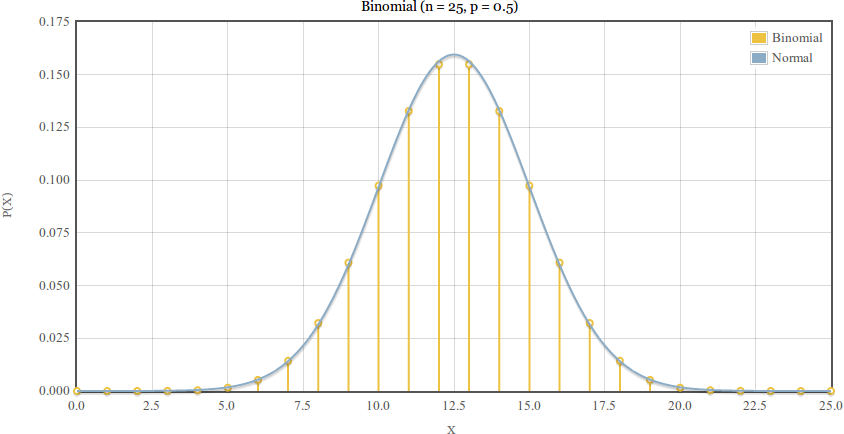
\includegraphics[width=\textwidth]{../images/binomial-normal-1.png}}
    \only<2>{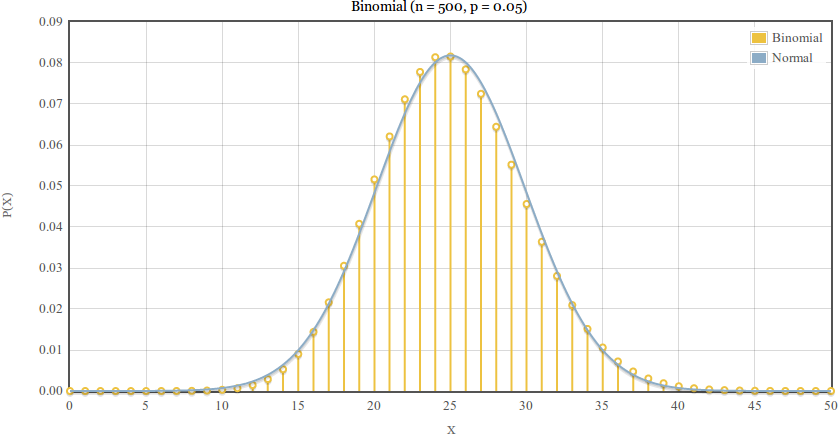
\includegraphics[width=\textwidth]{../images/binomial-normal-2.png}}
  \end{center}
}
\frame{ \frametitle{Introduction}
  However, when $n$ is medium and $p$ is extreme ...
  \begin{center}
    \only<1>{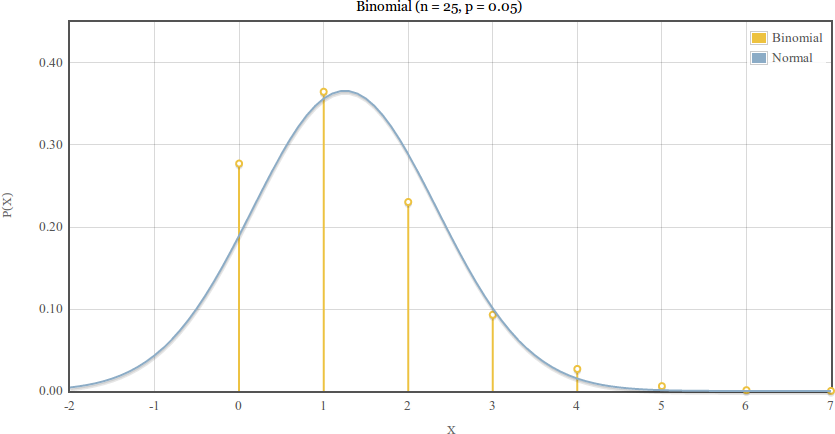
\includegraphics[width=\textwidth]{../images/binomial-normal-sn-1.png}}
    \only<2>{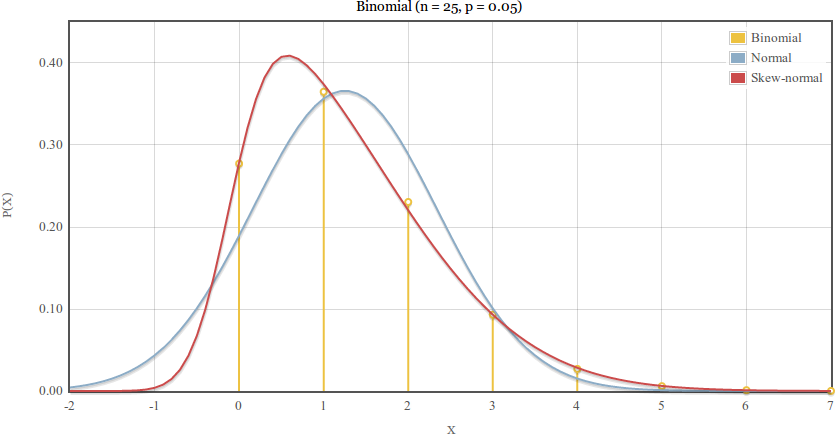
\includegraphics[width=\textwidth]{../images/binomial-normal-sn-2.png}}
    \only<3>{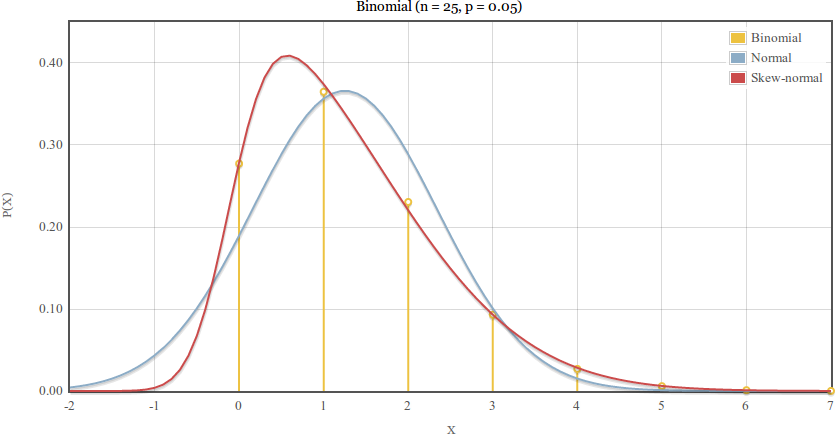
\includegraphics[width=\textwidth]{../images/binomial-normal-sn-3.png}}
  \end{center}
  \only<1>{the binomial is very skewed ...}
  \only<2>{and the normal approximation doesn't work very well.}
  \only<3>{Introducing ... the skew-normal distribution.}
}

%% Outline
\frame{ \frametitle{Outline}
  Today's itinerary:
  \begin{enumerate}[<+->]
    \item Skew-Normal distribution -- basic properties
    \item Method of Moments -- derive an approximation
    \item Accuracy -- compare to the normal approximation
  \end{enumerate}
}

% The Skew-Normal Distribution
\frame{ \frametitle{The Skew-Normal Distribution: Foundations}
  \begin{definition}[Skew-normal]
    Let $Y$ be a skew-normal distribution, with location parameter $\mu \in
    \R$, scale parameter $\sigma > 0$, and shape parameter $\lambda \in \R$.
    Then $Y$ has pdf

    \begin{equation*}
      f(x|\mu, \sigma, \lambda) = \frac2\sigma \cdot \phi \left( \frac{x-\mu}{\sigma} \right) \cdot \Phi \left( \frac{\lambda(x-\mu)}{\sigma} \right), \quad x \in \R,
    \end{equation*}

    where $\phi$ is the standard normal pdf and $\Phi$ is the standard normal
    cdf.

    \vsep
    We write $Y \sim SN(\mu, \sigma, \lambda)$.
  \end{definition}
}
\frame{ \frametitle{The Skew-Normal Distribution: Foundations}
  \tikzstyle{na} = [baseline=-.5ex]

  So where did this funny-looking pdf come from? ...
  \pause
  \begin{lem*}
    If $f_0$ is a one-dimensional probability density function symmetric about
    0, and $G$ is a one-dimensional distribution function such that $G'$ exists
    and is a density symmetric about 0, then
    % Below we mix an ordinary equation with TikZ nodes. Note that we have to
    % adjust the baseline of the nodes to get proper alignment with the rest of
    % the equation.
    \begin{equation*}
      f(z) = 2 \; \cdot
            \tikz[baseline]{
                \node[fill=blue!20,anchor=base] (t1)
                {$f_0(z)$};
            } \cdot
            \tikz[baseline]{
                \node[fill=red!20,ellipse,anchor=base] (t2)
                {$G\{w(z)\}$};
            }
      \quad (-\infty < z < \infty)
    \end{equation*}
    is a density function for any odd function $w(\cdot)$. (Lemma 1,
    \citealp{azzalini})
  \end{lem*}
  \begin{itemize}
    \uncover<3->{
      \item Kernel
        \tikz[na] \node[coordinate] (n1) {};
    }
    \uncover<4->{
      \item CDF
        \tikz[na] \node[coordinate] (n2) {};
    }
  \end{itemize}

  % Now it's time to draw some edges between the global nodes. Note that we
  % have to apply the 'overlay' style.
  \begin{tikzpicture}[overlay]
    \path[->]<3-> (n1) edge [bend right] (t1);
    \path[->]<4-> (n2) edge [bend right] (t2);
  \end{tikzpicture}
}
\frame{ \frametitle{The Skew-Normal Distribution: Foundations}

  Basic properties:

  \begin{align*}
    E(Y) &= \mu + b \delta \sigma \\
    E(Y^2) &= \mu^2 + 2b \delta \mu \sigma + \sigma^2 \\
    E(Y^3) &= \mu^3 + 3 b \delta \mu^2 \sigma + 3 \mu \sigma^2 + 3 b \delta \sigma^3 - b \delta^3 \sigma^3 \\
    Var(Y) &= \sigma^2 (1 - b^2 \delta^2)
  \end{align*}

  where $b = \sqrt{\frac{2}{\pi}}$ and $\delta = \frac{\lambda}{\sqrt{1 +
  \lambda^2}}$. \citep{pewsey}
}
\frame{ \frametitle{The Skew-Normal Distribution: Foundations}

  What happens when $\lambda=0$?
  \pause
  \begin{align*}
    \uncover<+->{f(x|\mu, \sigma, \lambda=0) &= \frac2\sigma \cdot \phi \left( \frac{x-\mu}{\sigma} \right) \cdot \Phi(0) \\}
    \uncover<+->{&= \frac2\sigma \cdot \phi \left( \frac{x-\mu}{\sigma} \right) \cdot 0.5 \\}
    \uncover<+->{&= \frac1\sigma \cdot \phi \left( \frac{x-\mu}{\sigma} \right) \\}
    \uncover<+->{&= \frac{1}{\sqrt{2\pi}\sigma} \;\cdot\; \exp \left( -\frac{(x-\mu)^2}{2\sigma^2} \right),}
  \end{align*}
  \uncover<+->{which is the pdf of the normal distribution ($\mu$, $\sigma$).}
}
\frame{ \frametitle{The Skew-Normal Distribution: The Standard Skew-Normal}

  \begin{definition}[Standard skew-normal]
    The $SN(0,1,\lambda)$ distribution is called the standard skew-normal and
    has pdf

    \begin{equation*}
      f_Z(x|\lambda) = 2 \cdot \phi(x) \cdot \Phi (\lambda x), \quad x \in \R.
    \end{equation*}
  \end{definition}
  \pause

  Similar to the normal and standard normal, $Z = \frac{Y - \mu}{\sigma}$ and $Y
  = \sigma Z + \mu$.
}
\frame{ \frametitle{The Skew-Normal Distribution: The Standard Skew-Normal}
  \begin{property}[1]
    If $Z \sim SN(0, 1, \lambda)$, then $(-Z) \sim SN(0, 1, -\lambda)$.
  \end{property}
  \pause
  \begin{pf}
    \pause
    \begin{align*}
      \uncover<+->{f_{(-Z)}(x) &= f_Z(-x) \\}
      \uncover<+->{& = 2 \cdot \phi(-x) \cdot \Phi (-\lambda x) \\}
      \uncover<+->{& = 2 \cdot \phi(x) \cdot \Phi (-\lambda x),}
    \end{align*}
    \uncover<+->{which is the pdf of $SN(0, 1, -\lambda)$.}
  \end{pf}
}
\frame{ \frametitle{The Skew-Normal Distribution: The Standard Skew-Normal}
  \textit{Property 1}:\; $-SN(0, 1, \lambda) \sim SN(0, 1, -\lambda)$

  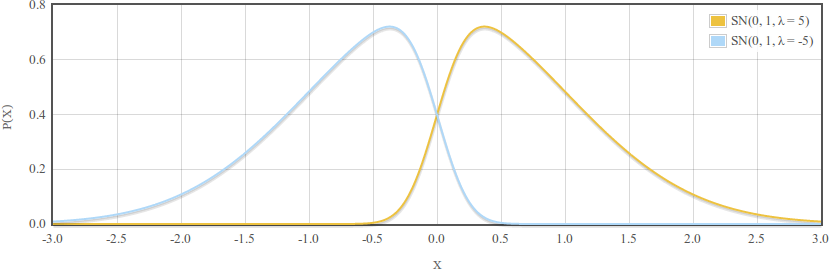
\includegraphics[width=\textwidth]{../images/std-sn-reflection.png}
}
\frame{ \frametitle{The Skew-Normal Distribution: The Standard Skew-Normal}
  \begin{property}[2]
    If $Z \sim SN(0, 1, \lambda)$, then $Z^2 \sim \chi^2_1$ (chi-square with 1 degree of freedom).
  \end{property}
  \pause
  \begin{pf}
    \pause
    We will use a result from page 161, \citet{azzalini}:

    If $Y \sim f_0$ and $Z \sim f$, then $|Y| \overset{d}{=} |Z|$, where the
    notation $\overset{d}{=}$ denotes equality in distribution.

    \pause
    Let $X \sim N(0,1)$. Since $X^2 \sim \chi^2_1$ and $|X| \overset{d}{=}
    |Z|$, then $Z^2 \sim \chi^2_1$.
  \end{pf}
}
\frame{ \frametitle{The Skew-Normal Distribution: The Standard Skew-Normal}
  \begin{property}[3]
    As $\lambda \to \pm \infty$, \thinspace $SN(0,1,\lambda)$ tends to the half normal distribution, $\pm |N(0,1)|$.
  \end{property}
  \pause
    Let $X \sim |N(0, 1)|$. Then
    \begin{equation*}
      f_X(x) =
      \begin{dcases*}
        0      & when $-\infty < x \leq 0$ \\
        2 \phi & when $0 < x < \infty$ 
      \end{dcases*}
      .
    \end{equation*}
}
% For some reason, I was obliged to split the following slide into 3 slides, to prevent bumping in between the images.
\frame{ \frametitle{The Skew-Normal Distribution: The Standard Skew-Normal}
  \textit{Property 3}: $SN(0, 1, \lambda) \rightarrow +|N(0,1)|$ as $\lambda \rightarrow \infty$:

  \only<1>{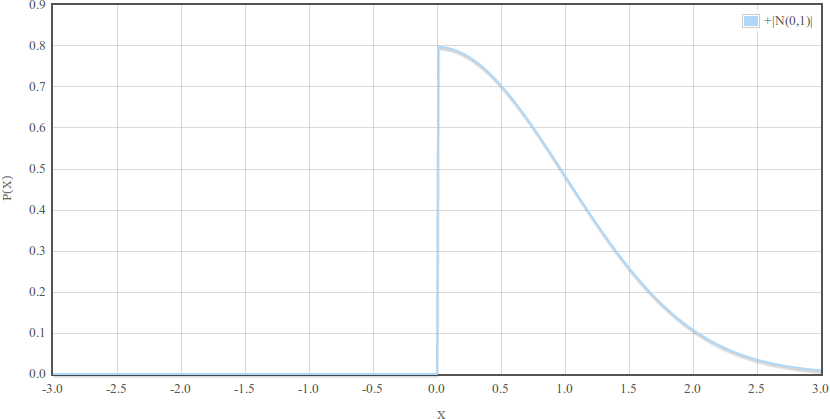
\includegraphics[width=\textwidth]{../images/positive-half-normal.png}}
}
\frame{ \frametitle{The Skew-Normal Distribution: The Standard Skew-Normal}
  \textit{Property 3}: $SN(0, 1, \lambda) \rightarrow +|N(0,1)|$ as $\lambda \rightarrow \infty$:

  \only<1>{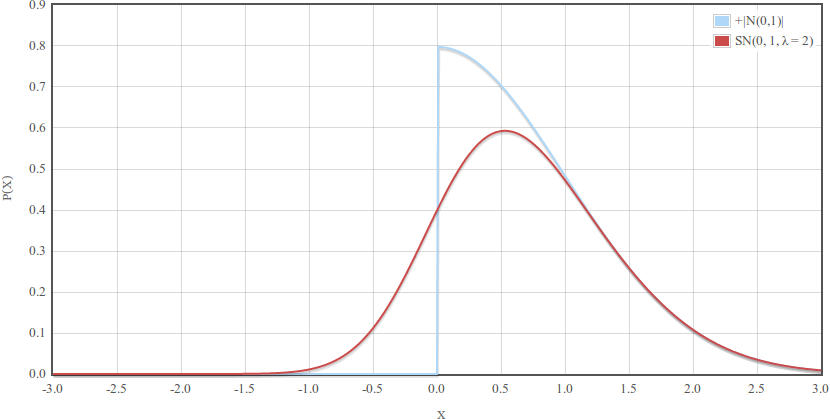
\includegraphics[width=\textwidth]{../images/std-sn-skew2.png}}
  \only<2>{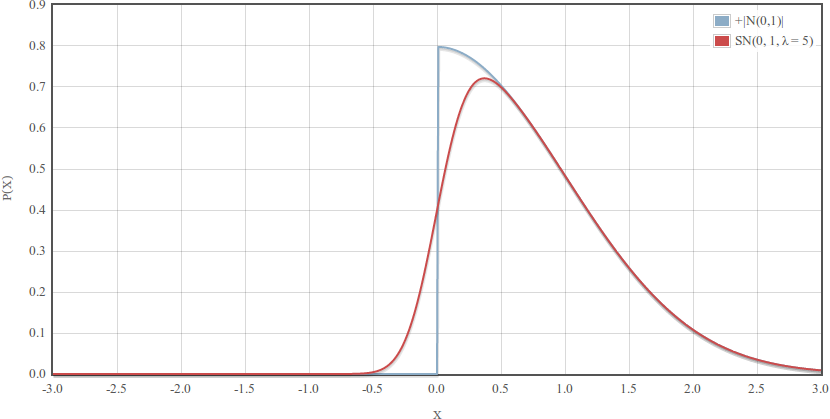
\includegraphics[width=\textwidth]{../images/std-sn-skew5.png}}
}
\frame{ \frametitle{The Skew-Normal Distribution: The Standard Skew-Normal}
  \textit{Property 3}: $SN(0, 1, \lambda) \rightarrow +|N(0,1)|$ as $\lambda \rightarrow \infty$:

  \only<1>{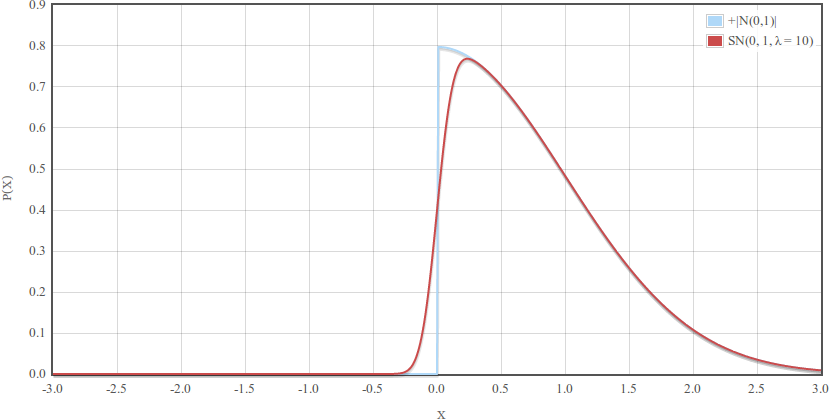
\includegraphics[width=\textwidth]{../images/std-sn-skew10.png}}
  \only<2>{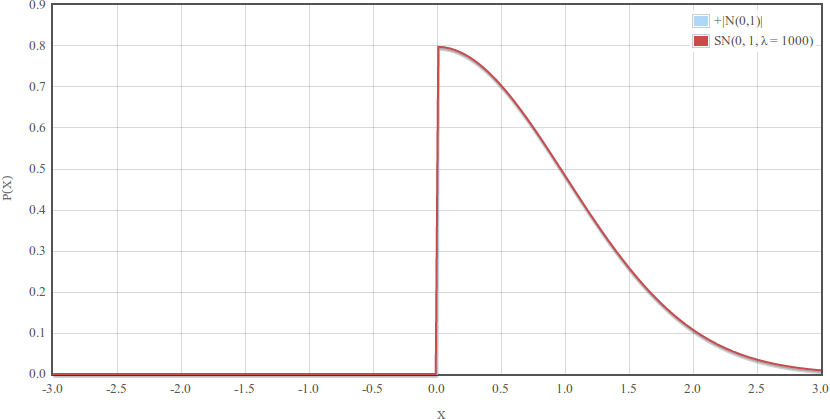
\includegraphics[width=\textwidth]{../images/std-sn-skew1000.png}}
}
% end
% Same bumping issue for this slide
\frame{ \frametitle{The Skew-Normal Distribution: The Standard Skew-Normal}
  \textit{Property 3}: $SN(0, 1, \lambda) \rightarrow -|N(0,1)|$ as $\lambda \rightarrow -\infty$:

  \only<1>{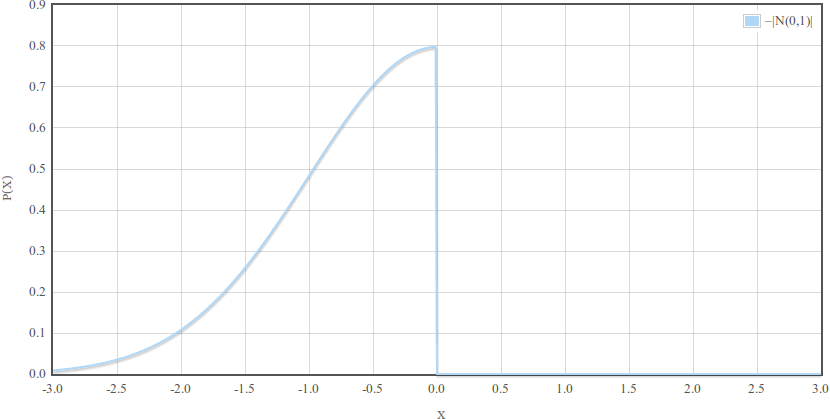
\includegraphics[width=\textwidth]{../images/negative-half-normal.png}}
}
\frame{ \frametitle{The Skew-Normal Distribution: The Standard Skew-Normal}
  \textit{Property 3}: $SN(0, 1, \lambda) \rightarrow -|N(0,1)|$ as $\lambda \rightarrow -\infty$:

  \only<1>{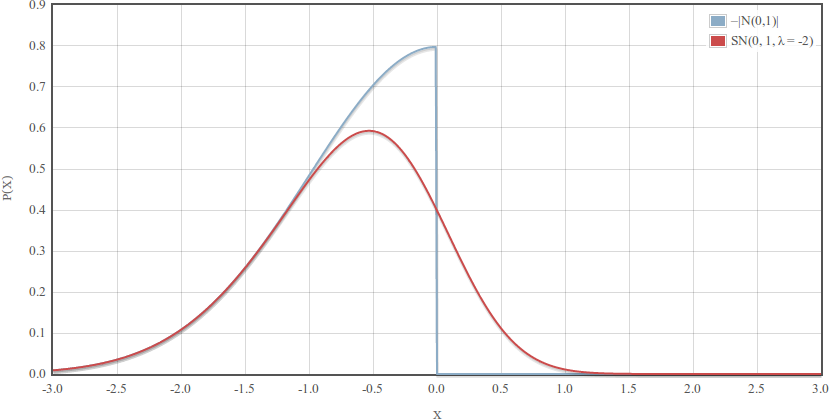
\includegraphics[width=\textwidth]{../images/std-sn-skewneg2.png}}
  \only<2>{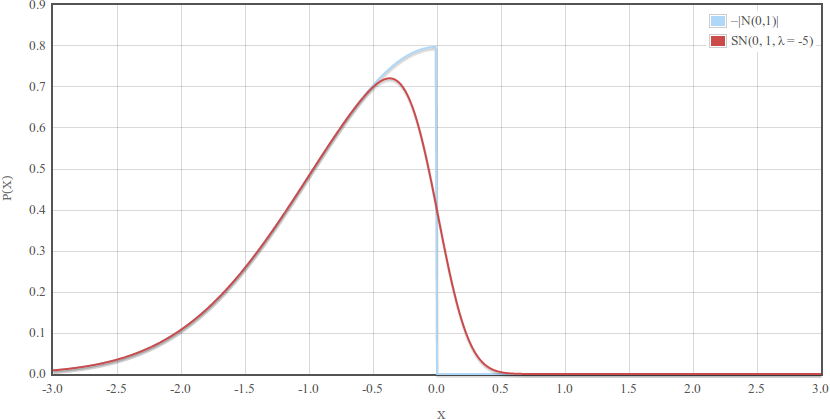
\includegraphics[width=\textwidth]{../images/std-sn-skewneg5.png}}
}
\frame{ \frametitle{The Skew-Normal Distribution: The Standard Skew-Normal}
  \textit{Property 3}: $SN(0, 1, \lambda) \rightarrow -|N(0,1)|$ as $\lambda \rightarrow -\infty$:

  \only<1>{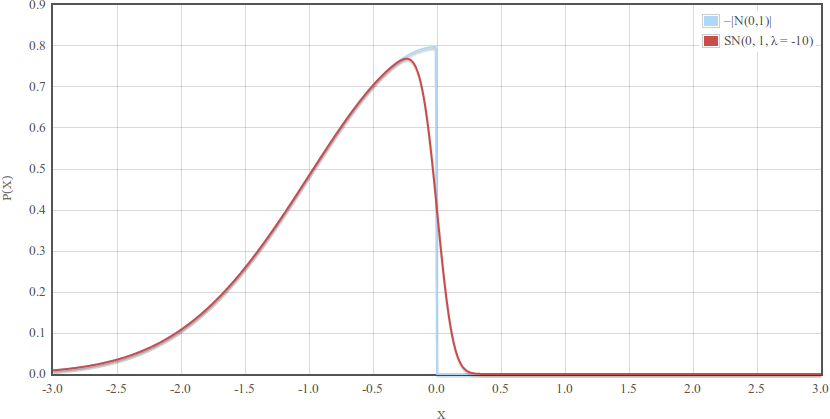
\includegraphics[width=\textwidth]{../images/std-sn-skewneg10.png}}
  \only<2>{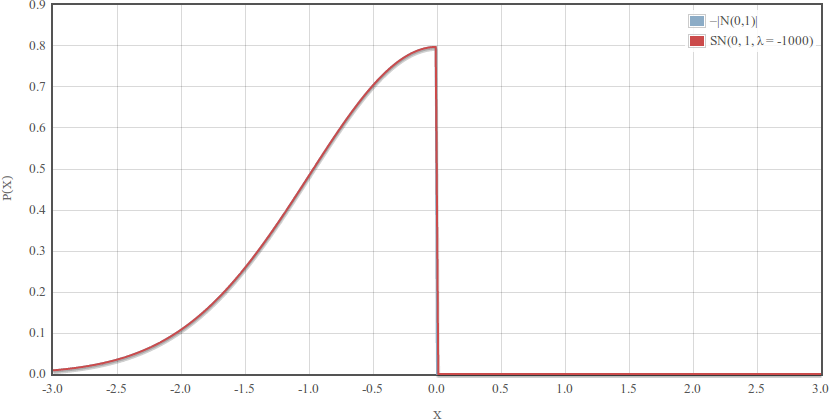
\includegraphics[width=\textwidth]{../images/std-sn-skewneg1000.png}}
}
% end
\frame{ \frametitle{The Skew-Normal Distribution: The Standard Skew-Normal}
  \begin{property}[4]
    The moment generating function of $SN(0,1,\lambda)$ is
    \begin{equation*}
      M(t|\lambda) = 2 \cdot \Phi (\delta t) \cdot e^{t^2/2},
    \end{equation*}
    where $\delta = \frac{\lambda}{\sqrt{1 + \lambda^2}}$ and $t \in (-\infty, \infty)$.
  \end{property}
  According to Equation 5 in \citet{azzalini}, the mgf of $SN(\mu, \sigma, \lambda)$ is
  \begin{equation*}
    M(t) \eq E\{e^{tY}\} \eq 2 \cdot \exp \left( \mu t + \frac{\sigma^2 t^2}{2} \right) \cdot \Phi(\delta \sigma t).
  \end{equation*}
  Our result follows.
}

% Method of Moments

\frame{ \frametitle{Method of Moments: Overview}
  Now we're going to derive the approximation!
  \pause

  Game plan:
  \pause
  \begin{enumerate}[<+->]
    \item Find the first three moments about the mean (central moments) of the binomial and the skew-normal.\\
          \pause
          \vsep
          What are central moments?: $E(X)$, $E([X - E(X)]^2)$, $E([X -
          E(X)]^3)$.
    \item Set them equal to each other.
    \item Take $n$ and $p$ to be constants; solve for $\mu$, $\sigma$, and $\lambda$.
  \end{enumerate}
}

%% The Central Moments of the Binomial
\frame{ \frametitle{Method of Moments: Central Moments of the Binomial}
  Let's start with the binomial ...
}
\frame{ \frametitle{Method of Moments: Central Moments of the Binomial}
  The first two central moments are just the mean and variance:
  \pause
  \begin{align*}
    E(B) &= np \\
    E([B - E(B)]^2) &= Var(B) = np(1-p)
  \end{align*}
}
\frame{ \frametitle{Method of Moments: Central Moments of the Binomial}
  The third one takes some elbow grease.
  \pause

  First we'll need to find $E(B^2)$ and $E(B^3)$.
}
\frame{ \frametitle{Method of Moments: Central Moments of the Binomial}
  \begin{align*}
    \uncover<+->{E(B^2) &= Var(B) + [E(B)]^2 \\}
    \uncover<+->{&= np(1-p) + n^2p^2 \\}
    \uncover<+->{&= np - np^2 + n^2p^2}
  \end{align*}
}
\frame{ \frametitle{Method of Moments: Central Moments of the Binomial}
  We will get $E(B^3)$ via the third factorial moment, E[B(B-1)(B-2)].
}
\frame{ \frametitle{Method of Moments: Central Moments of the Binomial}
  \begin{align*}
    \uncover<+->{&E[B(B-1)(B-2)] \\}
    \uncover<+->{&= \sum_{x=0}^n x (x-1) (x-2) \cdot \left\{ \binom{n}{x} p^x q^{n-x} \right\} \\}
    \uncover<+->{&= \sum_{x=3}^n x (x-1) (x-2) \cdot \left\{ \binom{n}{x} p^x q^{n-x} \right\} \\}
    \uncover<+->{&= \sum_{x=3}^n x(x-1)(x-2) \cdot \frac{n!}{x!\;(n-x)!} \; p^x q^{n-x} \\}
    \uncover<+->{&= \sum_{x=3}^n \frac{n!}{(x-3)!\;(n-x)!} \; p^x q^{n-x} \\}
    \uncover<+->{&= \sum_{x=3}^n n(n-1)(n-2) p^3 \cdot \frac{(n-3)!}{(x-3)!\;(n-x)!} \; p^{x-3}q^{n-x} \\}
  \end{align*}
}
\frame{ \frametitle{Method of Moments: Central Moments of the Binomial}
  Let $y=x-3$; then $x=y+3$, and $x=3$, $x=n \Ra y=0$, $y=n-3$:
  \pause
  \begin{align*}
    \uncover<+->{&= \sum_{x=3}^n n(n-1)(n-2) p^3 \cdot \frac{(n-3)!}{(x-3)!\;(n-x)!} \; p^{x-3}q^{n-x} \\}
    \uncover<+->{&= n(n-1)(n-2)p^3 \cdot \sum_{y=0}^{n-3} \frac{(n-3)!}{y!\;(n-(y+3))!} \; p^y q^{n-(y+3)} \\}
    \uncover<+->{&= n(n-1)(n-2)p^3 \cdot \underbrace {\sum_{y=0}^{n-3} \frac{(n-3)!}{y!\;((n-3)-y)!} \; p^y q^{(n-3)-y}}_{\mathclap{\textnormal{[pdf of $Bin(n-3,p)$ summed over its domain] = 1}}} \\}
    \uncover<+->{&= n(n-1)(n-2)p^3 \\}
    \uncover<+->{&= n^3p^3 - 3n^2p^3 + 2np^3}
  \end{align*}
}
\frame{ \frametitle{Method of Moments: Central Moments of the Binomial}
  To get $E(B^3)$, we expand the left side of the previous equation:
  \pause
  \begin{align*}
    \uncover<+->{&E[B(B-1)(B-2)] \\}
    \uncover<+->{&= E \left[ B^3 - 3B^2 + 2B \right] \\}
    \uncover<+->{&= E(B^3) - 3E(B^2) + 2E(B) \\}
    \uncover<+->{&= E(B^3) - 3(np - np^2 + n^2p^2) + 2np \\}
    \uncover<+->{&= E(B^3) - 3np + 3np^2 - 3n^2p^2 + 2np \\}
    \uncover<+->{&= E(B^3) + 3np^2 - 3n^2p^2 - np}
  \end{align*}
}
\frame{ \frametitle{Method of Moments: Central Moments of the Binomial}
  Left side: $E(B^3) + 3np^2 - 3n^2p^2 - np$

  Right side: $n^3p^3 - 3n^2p^3 + 2np^3$
  \pause

  Set them equal and solve for $E(B^3)$:
  \pause
  \begin{align*}
    \uncover<+->{&E(B^3) + 3np^2 - 3n^2p^2 - np = n^3p^3 - 3n^2p^3 + 2np^3 \\}
    \uncover<+->{&\Rightarrow \qquad E(B^3) = n^3p^3 - 3n^2p^3 + 2np^3 - 3np^2 + 3n^2p^2 + np}
  \end{align*}
}
\frame{ \frametitle{Method of Moments: Central Moments of the Binomial}
  Now we can (finally!) compute the third central moment:
  \pause
  \begin{align*}
    \uncover<+->{&E \left( [B - E(B)]^3 \right) \\}
    \uncover<+->{&= E \left( B^3 - 3B^2 E(B) + 3B [E(B)]^2 - [E(B)]^3 \right) \\}
    \uncover<+->{&= E(B^3) - 3 E(B^2) E(B) + 3 E(B) [E(B)]^2 - [E(B)]^3 \\}
    \uncover<+->{&= E(B^3) - 3 E(B^2) E(B) + 2 [E(B)]^3 \\}
    \uncover<+->{&= (n^3p^3 - 3n^2p^3 + 2np^3 - 3np^2 + 3n^2p^2 + np) \\
                 &\quad - 3(np - np^2 + n^2p^2)(np) + 2(np)^3 \\}
    \uncover<+->{&= \cancel{n^3p^3} - \cancel{3n^2p^3} + 2np^3 - 3np^2 + \cancel{3n^2p^2} + np \\
                 &\quad - \cancel{3n^2p^2} + \cancel{3n^2p^3} - \cancel{3n^3p^3} + \cancel{2n^3p^3} \\}
    \uncover<+->{&= 2np^3 - 3np^2 + np \\}
    \uncover<+->{&= np(p-1)(2p-1)}
  \end{align*}
}
\frame{ \frametitle{Method of Moments: Central Moments of the Binomial}
  Let's restate our results:
  \begin{align*}
    E(B) &= np, \\
    E([B - E(B)]^2) &= np(1-p), \\
    E([B - E(B)]^3) &= np(p-1)(2p-1)
  \end{align*}
}

%% The Central Moments of the Skew-Normal
\frame{ \frametitle{Method of Moments: Central Moments of the Skew-Normal}
  Now lets move on to skew-normal ...
}
\frame{ \frametitle{Method of Moments: Central Moments of the Skew-Normal}
  Again, the first and second central moments are the mean and variance.
  \pause
  \begin{align*}
    E(Y) &= \mu + b \delta \sigma \\
    Var(Y) &= \sigma^2 (1 - b^2 \delta^2)
  \end{align*}
}
\frame{ \frametitle{Method of Moments: Central Moments of the Skew-Normal}
  Again, the third one is a little harder:
  \pause
  \begin{align*}
    \uncover<+->{&E([Y - E(Y)]^3) \\}
    \uncover<+->{&= E(Y^3) - 3E(Y^2)E(Y) + 2[E(Y)]^3 \\}
    \uncover<+->{&= (\mu^3 + 3 b \delta \mu^2 \sigma + 3 \mu \sigma^2 + 3 b \delta \sigma^3 - b \delta^3 \sigma^3) \\
                 &\quad - 3 (\mu^2 + 2b \delta \mu \sigma + \sigma^2) (\mu + b \delta \sigma) + 2\;(\mu + b \delta \sigma)^3 \\}
    \uncover<+->{&= \cancel{\mu^3} + \cancel{3 b \delta \mu^2 \sigma} + \cancel{3 \mu \sigma^2} + \cancel{3 b \delta \sigma^3} - b \delta^3 \sigma^3 - \cancel{3 \mu^3} - \cancel{3 b \delta \mu^2 \sigma} \\
                 &\quad - \cancel{6 b \delta \mu^2 \sigma} - \cancel{6 b^2 \delta^2 \mu \sigma^2} - \cancel{3 \mu \sigma^2} - \cancel{3 b \delta \sigma^3} + \cancel{2 \mu^3} + \cancel{6 b \delta \mu^2 \sigma} \\
                 &\quad + \cancel{6 b^2 \delta^2 \mu \sigma^2} + 2 b^3 \delta^3 \sigma^3 \\}
    \uncover<+->{&= 2 b^3 \delta^3 \sigma^3 - b \delta^3 \sigma^3 \\}
    \uncover<+->{&= b \delta^3 \sigma^3 (2b^2 - 1)}
  \end{align*}
}
\frame{ \frametitle{Method of Moments: Central Moments of the Skew-Normal}
  Our results, restated:
  \begin{alignat*}{4}
    E(Y) &= \mu + b \delta \sigma \;&=&\; \mu + \sigma \cdot \sqrt{\frac{2}{\pi}} \cdot \frac{\lambda}{\sqrt{1 + \lambda^2}} \\
    E([Y - E(Y)]^2) &= \sigma^2 (1 - b^2 \delta^2) \;&=&\; \sigma^2 \left( 1 - \frac{2}{\pi} \cdot \frac{\lambda^2}{1 + \lambda^2} \right) \\
    E([Y - E(Y)]^3) &= b \delta^3 \sigma^3 (2b^2 - 1) \;&=&\; \sigma^3 \sqrt{\frac{2}{\pi}} \left( \frac{\lambda}{\sqrt{1 + \lambda^2}} \right)^3 \left( \frac{4}{\pi} - 1 \right)
  \end{alignat*}
}

%% Deriving an Approximation
\frame{ \frametitle{Method of Moments: Deriving an Approximation}
  Set the central moments of the binomial equal to the central moments of the skew-normal:
  \pause
  \begin{subequations}
    \begin{align}
      \uncover<+->{np &= \mu + \sigma \cdot \sqrt{\frac{2}{\pi}} \cdot \frac{\lambda}{\sqrt{1 + \lambda^2}} \label{eq:first-moment-set} \\}
      \uncover<+->{np(1-p) &= \sigma^2 \left( 1 - \frac{2}{\pi} \cdot \frac{\lambda^2}{1 + \lambda^2} \right) \label{eq:second-moment-set} \\}
      \uncover<+->{np(p-1)(2p-1) &= \sigma^3 \sqrt{\frac{2}{\pi}} \left( \frac{\lambda}{\sqrt{1 + \lambda^2}} \right)^3 \left( \frac{4}{\pi} - 1 \right) \label{eq:third-moment-set} \\}
      \notag
    \end{align}
  \end{subequations}
}
\frame{ \frametitle{Method of Moments: Deriving an Approximation}
  To get $\lambda$, divide the cube of \eqref{eq:second-moment-set} by the
  square of \eqref{eq:third-moment-set}:
  \pause
  \begin{align}
    \uncover<+->{\frac{\sigma^6 \left( 1 - \frac{2}{\pi} \cdot \frac{\lambda^2}{1 + \lambda^2} \right)^3}{\sigma^6 \cdot \frac{2}{\pi} \left( \frac{\lambda}{\sqrt{1 + \lambda^2}} \right)^6 \left(
                 \frac{4}{\pi} - 1 \right)^2} &= \frac{n^3p^3(1-p)^3}{n^2p^2(p-1)^2(2p-1)^2} \nonumber \\}
    \uncover<+->{\Rightarrow \quad \frac{\left( 1 - \frac{2}{\pi} \cdot \frac{\lambda^2}{1+\lambda^2} \right)^3}{\frac{2}{\pi} \left( \frac{\lambda^2}{1+\lambda^2} \right)^3 \left( \frac{4}{\pi} - 1
                 \right)^2} &= \frac{np(1-p)}{(1-2p)^2} \label{eq:solving-for-lambda}}
  \end{align}
}
\frame{ \frametitle{Method of Moments: Deriving an Approximation}
  Equation \eqref{eq:solving-for-lambda} can be solved for $\lambda^2$.
  \pause

  Then take $\lambda$ to be
  \begin{equation*}
    \lambda = \textnormal{\{sign of $(1-2p)$\}} \sqrt{\lambda^2}.
  \end{equation*}
}
\frame{ \frametitle{Method of Moments: Deriving an Approximation}
  Once you have $\lambda$, solve for $\sigma$ and then $\mu$.
  \pause
  \begin{equation*}
    \uncover<+->{np(1-p) = \sigma^2 \left( 1 - \frac{2}{\pi} \cdot \frac{\lambda^2}{1 + \lambda^2} \right) \quad\Rightarrow\quad
                 \sigma = \sqrt{\frac{np(1-p)}{1 - \frac{2}{\pi} \cdot \frac{\lambda^2}{1 + \lambda^2}}}}
  \end{equation*}
  \begin{equation*}
    \uncover<+->{np = \mu + \sigma \cdot \sqrt{\frac{2}{\pi}} \cdot \frac{\lambda}{\sqrt{1 + \lambda^2}} \quad\Rightarrow\quad
                 \mu = np - \sigma \cdot \sqrt{\frac{2}{\pi}} \cdot \frac{\lambda}{\sqrt{1 + \lambda^2}}}
  \end{equation*}
}
\frame{ \frametitle{Method of Moments: Deriving an Approximation}
  When $p = 0.5$, the binomial is symmetric, so $\lambda=0$.
  \pause

  This takes us back to the usual normal approximation:
  \pause
  \begin{align*}
    \uncover<+->{\sigma &= \sqrt{\frac{np(1-p)}{1 - \frac{2}{\pi} \cdot \frac{0^2}{1 + 0^2}}} = \sqrt{\frac{np(1-p)}{1}} = \sqrt{np(1-p)} \\}
    \uncover<+->{\mu &= np - \sigma \cdot \sqrt{\frac{2}{\pi}} \cdot \frac{0}{\sqrt{1 + 0^2}}  = np - 0 = np}
  \end{align*}
}

%% Restrictions
\frame{ \frametitle{Method of Moments: Restrictions}
  Unfortunately, though better than the normal approximation, our skew-normal method isn't universal.
  \pause

  To be able to solve for $\lambda$, we must put a few restrictions on $n$ and $p$.
}
\frame{ \frametitle{Method of Moments: Restrictions}
  Let $u = \frac{\lambda^2}{1+\lambda^2}$ and $v = 1/u = \frac{1+\lambda^2}{\lambda^2}$.
  \pause

  \uncover<+->{Then we can rewrite \eqref{eq:solving-for-lambda}:
  \begin{gather*}
    \frac{\left( 1 - \frac{2}{\pi} \cdot \frac{\lambda^2}{1+\lambda^2} \right)^3}{\frac{2}{\pi} \left( \frac{\lambda^2}{1+\lambda^2} \right)^3 \left( \frac{4}{\pi} - 1 \right)^2} \\}
    \uncover<+->{\vdots \\
                 (magic) \\
                 \vdots \\}
    \uncover<+->{\left( v - \frac{2}{\pi} \right)^3 \left( \frac{\pi^3}{2(4-\pi)^2} \right) = g(v)}
  \end{gather*}
}
\frame{ \frametitle{Method of Moments: Restrictions}
  $g(v)$ is increasing in $v = \frac{1+\lambda^2}{\lambda^2} \geq 1$. \pause Therefore:
  \begin{equation*}
    \uncover<+->{\min_{v} g(v)} \uncover<+->{= g(1)} \uncover<+->{= \left( 1 - \frac{2}{\pi} \right)^3 \left( \frac{\pi^3}{2(4-\pi)^2} \right)} \uncover<+->{= 1.009524 \approx 1}
  \end{equation*}
}
\frame{ \frametitle{Method of Moments: Restrictions}
  To be able to solve \eqref{eq:solving-for-lambda} for $\lambda$, we must have
  \begin{align}
    \uncover<+->{\textnormal{\{right hand side of \eqref{eq:solving-for-lambda}\}} &\geq \textnormal{\{min of left hand side of \eqref{eq:solving-for-lambda}\}} \nonumber \\}
    \uncover<+->{\frac{np(1-p)}{(1-2p)^2} &\geq 1 \nonumber \\}
    \uncover<+->{np(1-p) &\geq (1-2p)^2. \label{eq:solving-the-restriction}}
  \end{align}
  \uncover<+->{From \eqref{eq:solving-the-restriction}, we can answer two questions:}
}
\frame{ \frametitle{Method of Moments: Restrictions}
  One:

  Given $p$, what is the least $n$ necessary?
  \pause
  \begin{equation*}
    n \geq \frac{(1-2p)^2}{p(1-p)}
  \end{equation*}
}
\frame{ \frametitle{Method of Moments: Restrictions}
  Least possible $n$, given a fixed $p$:
  \begin{center}
    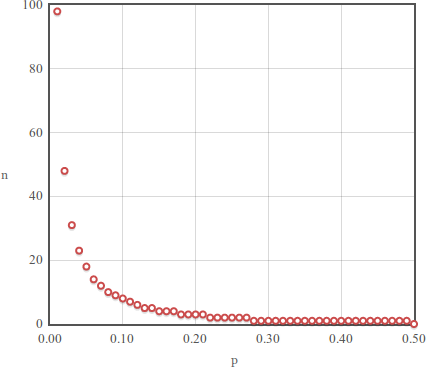
\includegraphics[width=0.7\textwidth]{../images/restriction-least-n.png}
  \end{center}
}
\frame{ \frametitle{Method of Moments: Restrictions}
  Two:

  Given $n$, what is the range of possible $p$'s?
  \pause
  \begin{equation*}
   \frac12 - \frac12 \sqrt{\frac{n}{n+4}} \; \leq \; p \; \leq \; \frac12 + \frac12 \sqrt{\frac{n}{n+4}}
  \end{equation*}
}
\frame{ \frametitle{Method of Moments: Restrictions}
  Range of possible $p$, given a fixed $n$:
  \begin{center}
    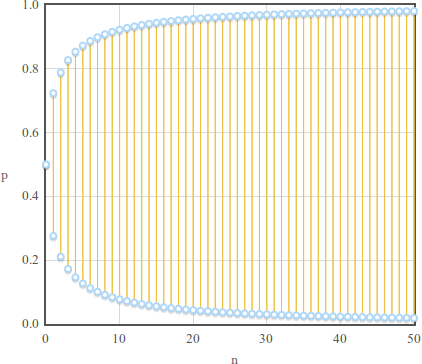
\includegraphics[width=0.8\textwidth]{../images/restriction-p-range.png}
  \end{center}
}

% Demonstrating Improved Accuracy

\frame{ \frametitle{Demonstrating Improved Accuracy}
  We have an approximation!!

  But is it more accurate? ... \pause Answer: Yes!
}

%% Visual Inspection
\frame{ \frametitle{Demonstrating Improved Accuracy: Visual}
  The easiest way of gauging accuracy is by visual inspection.
}
\frame{ \frametitle{Demonstrating Improved Accuracy: Visual}
  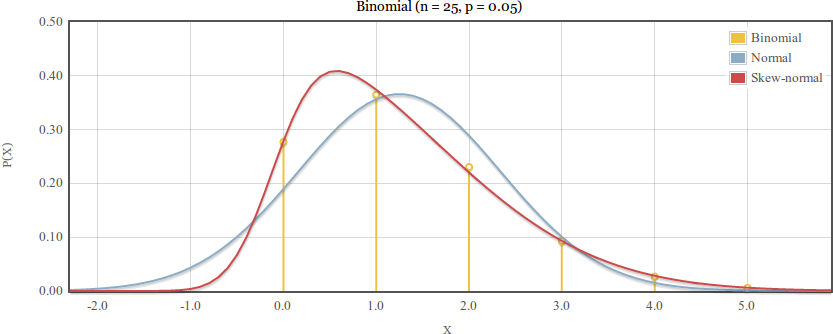
\includegraphics[width=\textwidth]{../images/comparison-n25-p005.png}
}
\frame{ \frametitle{Demonstrating Improved Accuracy: Visual}
  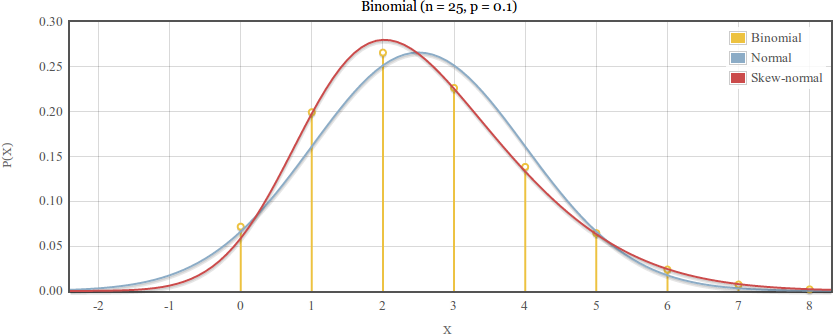
\includegraphics[width=\textwidth]{../images/comparison-n25-p01.png}
}
\frame{ \frametitle{Demonstrating Improved Accuracy: Visual}
  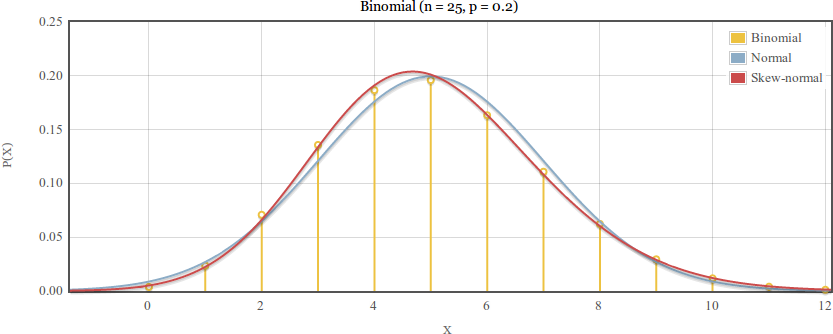
\includegraphics[width=\textwidth]{../images/comparison-n25-p02.png}
}
\frame{ \frametitle{Demonstrating Improved Accuracy: Visual}
  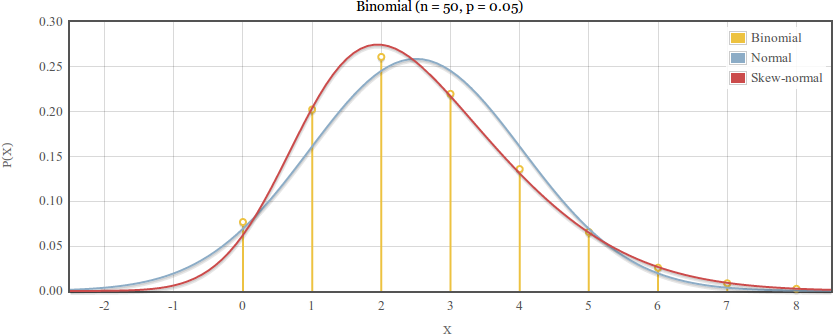
\includegraphics[width=\textwidth]{../images/comparison-n50-p005.png}
}
\frame{ \frametitle{Demonstrating Improved Accuracy: Visual}
  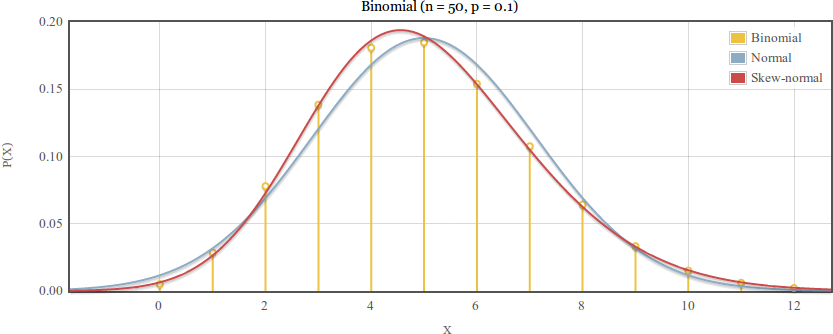
\includegraphics[width=\textwidth]{../images/comparison-n50-p01.png}
}
\frame{ \frametitle{Demonstrating Improved Accuracy: Visual}
  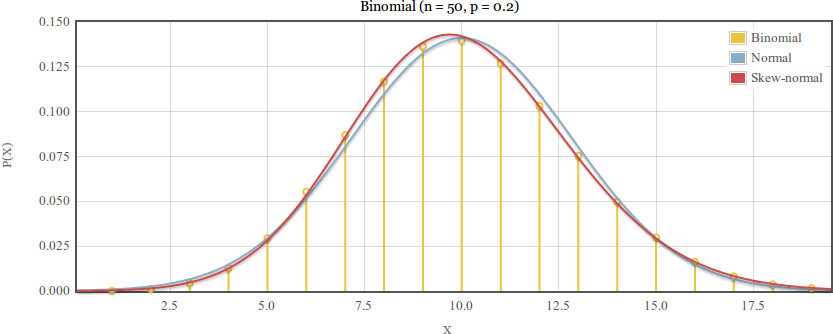
\includegraphics[width=\textwidth]{../images/comparison-n50-p02.png}
}
\frame{ \frametitle{Demonstrating Improved Accuracy: Visual}
  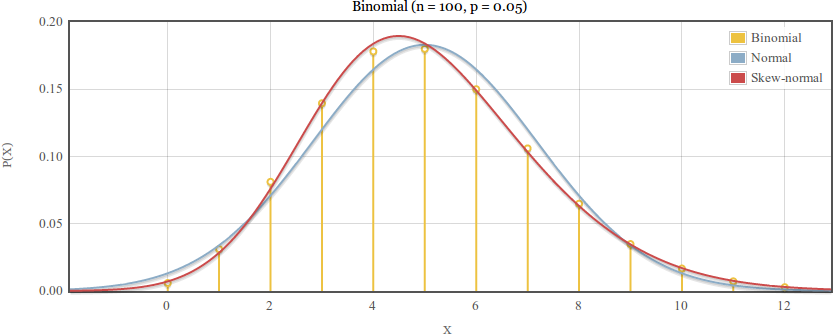
\includegraphics[width=\textwidth]{../images/comparison-n100-p005.png}
}
\frame{ \frametitle{Demonstrating Improved Accuracy: Visual}
  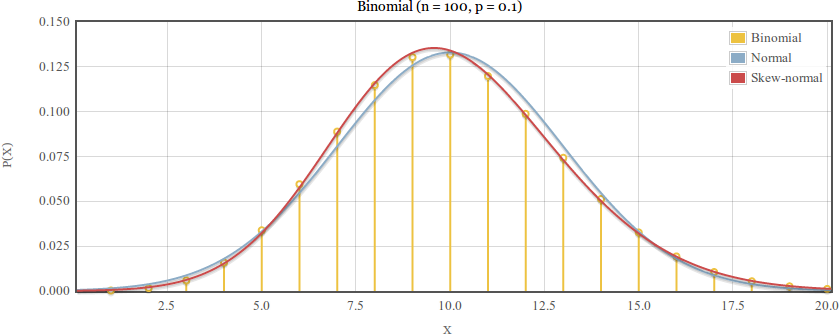
\includegraphics[width=\textwidth]{../images/comparison-n100-p01.png}
}
\frame{ \frametitle{Demonstrating Improved Accuracy: Visual}
  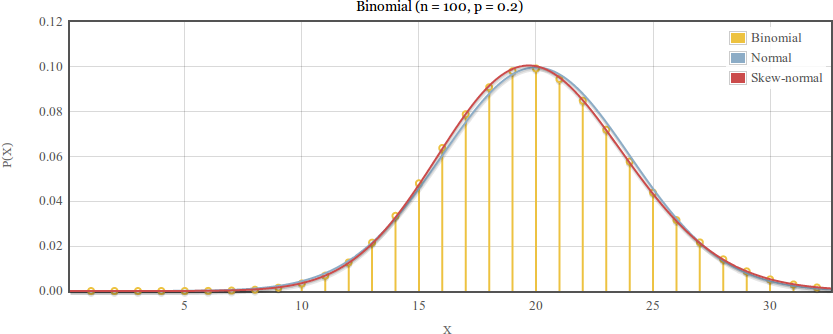
\includegraphics[width=\textwidth]{../images/comparison-n100-p02.png}
}

%% MABS
\frame{ \frametitle{Demonstrating Improved Accuracy: MABS}
  A more numerical way of gauging accuracy is the $MABS$, defined by \citet{mabs} as
  \begin{equation*}
    \textnormal{MABS}(n, p) \eq \max_{k \in \{0, 1,...,n\}} \left| F_{B(n,p)} (k) -  F_{\textnormal{appr}(n,p)}(k + 0.5) \right|.
  \end{equation*}
}
\frame{ \frametitle{Demonstrating Improved Accuracy: MABS}
  MABS as a function of $p$, with fixed $n=25$:

  \begin{center}
    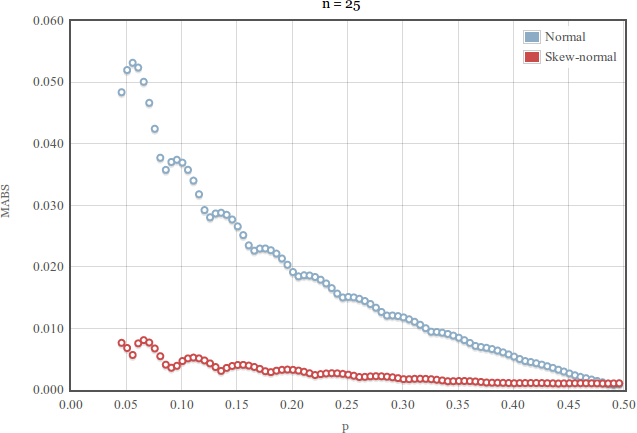
\includegraphics[width=0.8\textwidth]{../images/mabs-fixed-n25.png}
  \end{center}
}
\frame{ \frametitle{Demonstrating Improved Accuracy: MABS}
  MABS as a function of $p$, with fixed $n=100$:

  \begin{center}
    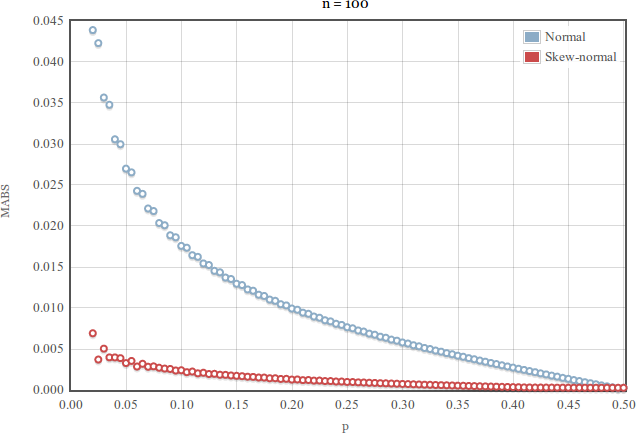
\includegraphics[width=0.8\textwidth]{../images/mabs-fixed-n100.png}
  \end{center}
}
\frame{ \frametitle{Demonstrating Improved Accuracy: MABS}
  MABS as a function of $n$, with fixed $p=0.05$:

  \begin{center}
    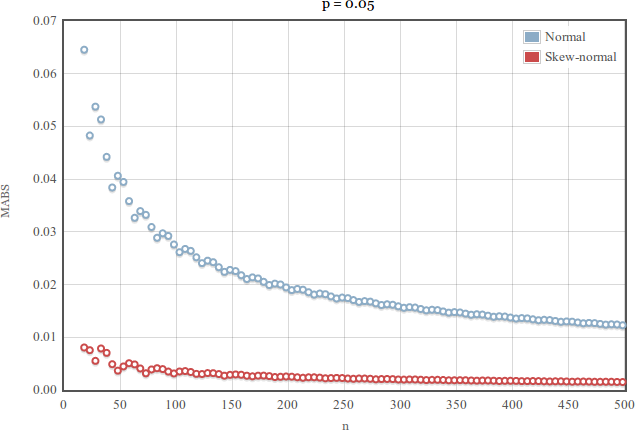
\includegraphics[width=0.8\textwidth]{../images/mabs-fixed-p005.png}
  \end{center}
}
\frame{ \frametitle{Demonstrating Improved Accuracy: MABS}
  MABS as a function of $n$, with fixed $p=0.1$:

  \begin{center}
    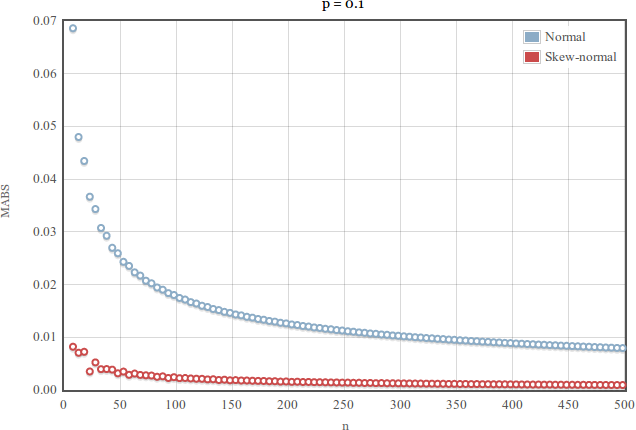
\includegraphics[width=0.8\textwidth]{../images/mabs-fixed-p01.png}
  \end{center}
}

\begin{frame}[shrink=47]{Resources}
  \vsep
  \vsep

  Estimations of $SN(\mu, \sigma, \lambda)$ for $Bin(n,p)$
  \vsep

  \renewcommand{\arraystretch}{1.3}
  \begin{tabular}
    { r r | r@{}r@{,\;}r@{,\;}r@{}l r@{}r@{,\;}r@{,\;}r@{}l r@{}r@{,\;}r@{,\;}r@{}l r@{}r@{,\;}r@{,\;}r@{}l r@{}r@{,\;}r@{,\;}r@{}l }
    \hline \hline
    & & \multicolumn{5}{c}{} & \multicolumn{5}{c}{} & \multicolumn{5}{c}{$n$} & \multicolumn{5}{c}{} & \multicolumn{5}{c}{}\\
    \multirow{20}{*}{$p$} & & \multicolumn{5}{c}{25} & \multicolumn{5}{c}{50} & \multicolumn{5}{c}{100} & \multicolumn{5}{c}{250} & \multicolumn{5}{c}{500} \\
    \hline
    & 0.05 & ( & -0.11 & 1.74 & 4.56 & ) & ( & 0.79 & 2.30 & 2.54 & ) & ( & 2.85 & 3.06 & 1.86 & ) & ( & 9.58 & 4.52 & 1.38 & ) & ( & 21.32 & 6.11 & 1.15 & ) \\
    & 0.10 & ( & 0.89 & 2.20 & 2.31 & ) & ( & 2.97 & 2.94 & 1.74 & ) & ( & 7.44 & 3.94 & 1.40 & ) & ( & 21.53 & 5.88 & 1.10 & ) & ( & 45.62 & 8.01 & 0.94 & ) \\
    & 0.15 & ( & 2.02 & 2.49 & 1.79 & ) & ( & 5.32 & 3.34 & 1.43 & ) & ( & 12.25 & 4.51 & 1.19 & ) & ( & 33.77 & 6.77 & 0.96 & ) & ( & 70.30 & 9.27 & 0.82 & ) \\
    & 0.20 & ( & 3.23 & 2.67 & 1.50 & ) & ( & 7.76 & 3.61 & 1.24 & ) & ( & 17.18 & 4.89 & 1.04 & ) & ( & 46.18 & 7.39 & 0.85 & ) & ( & 95.18 & 10.16 & 0.74 & ) \\
    & 0.25 & ( & 4.49 & 2.79 & 1.29 & ) & ( & 10.28 & 3.78 & 1.09 & ) & ( & 22.20 & 5.15 & 0.93 & ) & ( & 58.71 & 7.83 & 0.76 & ) & ( & 120.22 & 10.80 & 0.67 & ) \\
    & 0.30 & ( & 5.80 & 2.85 & 1.12 & ) & ( & 12.86 & 3.88 & 0.95 & ) & ( & 27.31 & 5.32 & 0.82 & ) & ( & 71.34 & 8.12 & 0.68 & ) & ( & 145.39 & 11.24 & 0.60 & ) \\
    & 0.35 & ( & 7.17 & 2.86 & 0.96 & ) & ( & 15.50 & 3.92 & 0.83 & ) & ( & 32.49 & 5.39 & 0.72 & ) & ( & 84.09 & 8.28 & 0.60 & ) & ( & 170.70 & 11.50 & 0.53 & ) \\
    & 0.40 & ( & 8.59 & 2.83 & 0.80 & ) & ( & 18.23 & 3.89 & 0.70 & ) & ( & 37.76 & 5.39 & 0.61 & ) & ( & 96.96 & 8.32 & 0.51 & ) & ( & 196.18 & 11.60 & 0.45 & ) \\
    & 0.45 & ( & 10.12 & 2.73 & 0.61 & ) & ( & 21.08 & 3.79 & 0.53 & ) & ( & 43.21 & 5.29 & 0.47 & ) & ( & 110.07 & 8.23 & 0.40 & ) & ( & 221.93 & 11.54 & 0.35 & ) \\
    & 0.50 & ( & 12.50 & 2.50 & 0.00 & ) & ( & 25.00 & 3.54 & 0.00 & ) & ( & 50.00 & 5.00 & 0.00 & ) & ( & 125.00 & 7.91 & 0.00 & ) & ( & 250.00 & 11.18 & 0.00 & ) \\
    & 0.55 & ( & 14.88 & 2.73 & -0.61 & ) & ( & 28.92 & 3.79 & -0.53 & ) & ( & 56.79 & 5.29 & -0.47 & ) & ( & 139.93 & 8.23 & -0.40 & ) & ( & 278.07 & 11.54 & -0.35 & ) \\
    & 0.60 & ( & 16.41 & 2.83 & -0.80 & ) & ( & 31.77 & 3.89 & -0.70 & ) & ( & 62.24 & 5.39 & -0.61 & ) & ( & 153.04 & 8.32 & -0.51 & ) & ( & 303.82 & 11.60 & -0.45 & ) \\
    & 0.65 & ( & 17.83 & 2.86 & -0.96 & ) & ( & 34.50 & 3.92 & -0.83 & ) & ( & 67.51 & 5.39 & -0.72 & ) & ( & 165.91 & 8.28 & -0.60 & ) & ( & 329.30 & 11.50 & -0.53 & ) \\
    & 0.70 & ( & 19.20 & 2.85 & -1.12 & ) & ( & 37.14 & 3.88 & -0.95 & ) & ( & 72.69 & 5.32 & -0.82 & ) & ( & 178.66 & 8.12 & -0.68 & ) & ( & 354.61 & 11.24 & -0.60 & ) \\
    & 0.75 & ( & 20.51 & 2.79 & -1.29 & ) & ( & 39.72 & 3.78 & -1.09 & ) & ( & 77.80 & 5.15 & -0.93 & ) & ( & 191.29 & 7.83 & -0.76 & ) & ( & 379.78 & 10.80 & -0.67 & ) \\
    & 0.80 & ( & 21.77 & 2.67 & -1.50 & ) & ( & 42.24 & 3.61 & -1.24 & ) & ( & 82.82 & 4.89 & -1.04 & ) & ( & 203.82 & 7.39 & -0.85 & ) & ( & 404.82 & 10.16 & -0.74 & ) \\
    & 0.85 & ( & 22.98 & 2.49 & -1.79 & ) & ( & 44.68 & 3.34 & -1.43 & ) & ( & 87.75 & 4.51 & -1.19 & ) & ( & 216.23 & 6.77 & -0.96 & ) & ( & 429.70 & 9.27 & -0.82 & ) \\
    & 0.90 & ( & 24.11 & 2.20 & -2.31 & ) & ( & 47.03 & 2.94 & -1.74 & ) & ( & 92.56 & 3.94 & -1.40 & ) & ( & 228.47 & 5.88 & -1.10 & ) & ( & 454.38 & 8.01 & -0.94 & ) \\
    & 0.95 & ( & 25.11 & 1.74 & -4.56 & ) & ( & 49.21 & 2.30 & -2.54 & ) & ( & 97.15 & 3.06 & -1.86 & ) & ( & 240.42 & 4.52 & -1.38 & ) & ( & 478.68 & 6.11 & -1.15 & ) \\
  \end{tabular}
\end{frame}
\frame{ \frametitle{Resources}
  All values in my project were computed using a Python library, which is freely available online:

  http://github.com/joycetipping/skew-normal-capstone/
}

\begin{frame}[allowframebreaks]
  \frametitle{Bibliography}
  \nocite{*}
  \bibliography{../bibliography.bib}
  \bibliographystyle{plainnat}
\end{frame}
\end{document}
